\begin{event}{Atelier PARI/GP 2019}{AtelierPARI2019}{Bordeaux (FR),
2019-01-14 to 2019-01-18}{PS,UB,UV,UW}{36}{6}{http://pari.math.u-bordeaux.fr/Events/PARI2019/}


\textbf{\ODK implication.} \ODK participants: B. Allombert, K. Belabas, J.
Cremona, V. Delecroix, J.  Demeyer, L. de Feo.

\ODK provided the main funding source for the workshop (accommodation,
subsistence and some travel expenses), for about 13k\euro.

\textbf{Event summary.} The 12th Atelier PARI/GP took place in Bordeaux
(France) from january 14h to 18th.

There were 57 registered participants from 31 different institutions
(no registration fees).

A typical day of the workshop had introductory talks and tutorials
in the morning; afternoons allowed ample time for hacking sessions,
discussions and training.

The Atelier featured 10 morning talks on mathematical topics and
implementation projects including 4 talks by \ODK members
\begin{itemize}
\item Bill Allombert ``New GP features'' and ``Parallel GP programming''.
\item John Cremona ``Computing classical modular forms for the LMFDB''.
\item Jeroen Demeyer ``\texttt{cypari2}: Python bindings for PARI/GP''.
\end{itemize}

Slides for all talks are available at
\url{http://pari.math.u-bordeaux.fr/Events/PARI2019/}

\textbf{Results and impact.} The workshop was productive and a successful
teaching and dissemination event; 12 participants came from developping
countries (Algeria, Djibouti, Lebanon, Morroco, Senegal, Tunisia,
Turkey).

It provided final feedback on recent PARI/GP developments that paved the way
for the release of \texttt{pari-2.12-alpha} (2019/06).

\begin{figure}[ht]
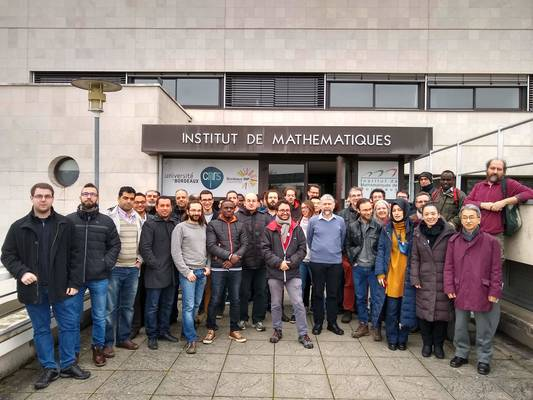
\includegraphics[scale=0.5]{pari2019.jpg}
\caption*{PARI/GP Atelier 2019 in Bordeaux}
\end{figure}

\end{event}
